%\title{Исследование производственных систем с маршрутизацией, зависящей от состояния}
%\author{Салин Роман Владимирович}
%\institute{САРАТОВСКИЙ ГОСУДАРСТВЕННЫЙ УНИВЕРСИТЕТ ИМЕНИ Н.Г. ЧЕРНЫШЕВСКОГО}
%\date{Саратов, 2014}

\begin{frame}[plain]
\begin{center}
Министерство образования и науки Российской Федерации\\
САРАТОВСКИЙ ГОСУДАРСТВЕННЫЙ УНИВЕРСИТЕТ\\
ИМЕНИ Н.Г. ЧЕРНЫШЕВСКОГО
\end{center}

%\vspace{0.5cm}
%\begin{flushright}
%\parbox{6.8cm}{
%\raggedright
%  Кафедра системного анализа \\ и автоматического управления
%}
%\end{flushright}

\vfill

\begin{center}
\textbf{Исследование производственных систем с маршрутизацией,\\зависящей от состояния}\\
\medskip
ВЫПУСКНАЯ КВАЛИФИКАЦИОННАЯ РАБОТА СПЕЦИАЛИСТА
\end{center}
\begin{flushleft}
студента 5 курса 511 группы\\
специальности 010501 --- прикладная математика и информатика\\
факультета компьютерных наук и информационных технологий\\
Салина Романа Владимировича
\end{flushleft}

\vfill

\noindent
\begin{flushleft}
Научный руководитель\\
доцент, к.ф.-м.н. \hfill В. И. Долгов\\
\end{flushleft}

\vfill

\begin{center}
Саратов 2014
\end{center}
\end{frame}

% ------------------------------------------------------------------- %

\begin{frame} \frametitle{Цели и задачи дипломной работы}
\begin{itemize}
\item исследование производственных систем с маршрутизацией, зависящей от состояния;
\item разработка алгоритма метода анализа производственных систем с маршрутизацией, зависящей от состояния;
\item программная реализация алгоритма;
\item проведение численных экспериментов с разработанной программой
\end{itemize}
\end{frame}

% ------------------------------------------------------------------- %

\begin{frame} \frametitle{Производственные системы с маршрутизацией, зависящей от состояния}

\end{frame}

% ------------------------------------------------------------------- %

\begin{frame} \frametitle{Производственные системы с маршрутизацией, зависящей от состояния}
\begin{figure}[H]
  \centering
  \includegraphics[width=0.9\textwidth]{fms}
  \label{fig:main}
\end{figure}
\end{frame}

% ------------------------------------------------------------------- %

\begin{frame} \frametitle{Интерфейс программы}
\begin{figure}[H]
  \centering
  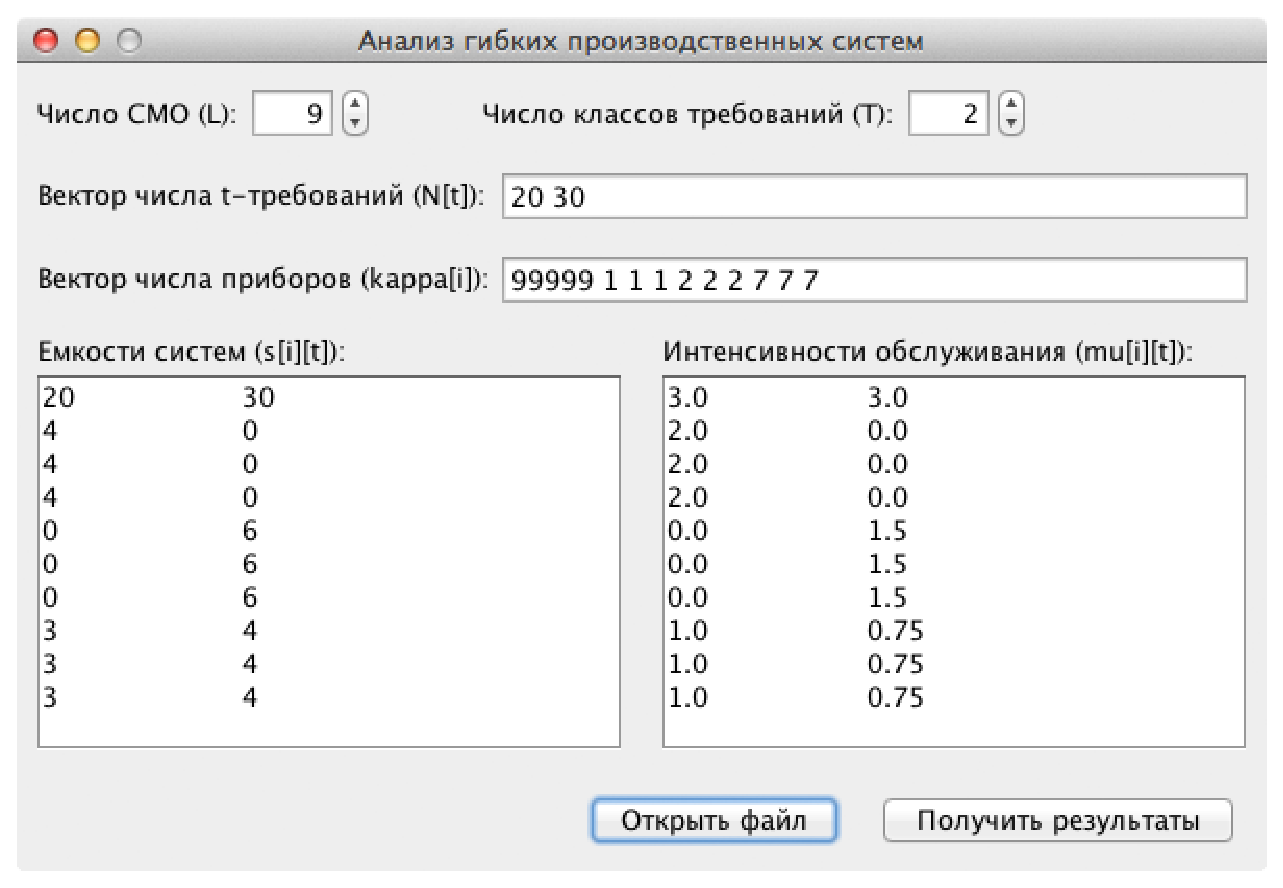
\includegraphics[width=0.9\textwidth]{main}
  \label{fig:main}
\end{figure}
\end{frame}

% ------------------------------------------------------------------- %

\begin{frame} \frametitle{Интерфейс программы}
\begin{figure}[H]
  \centering
  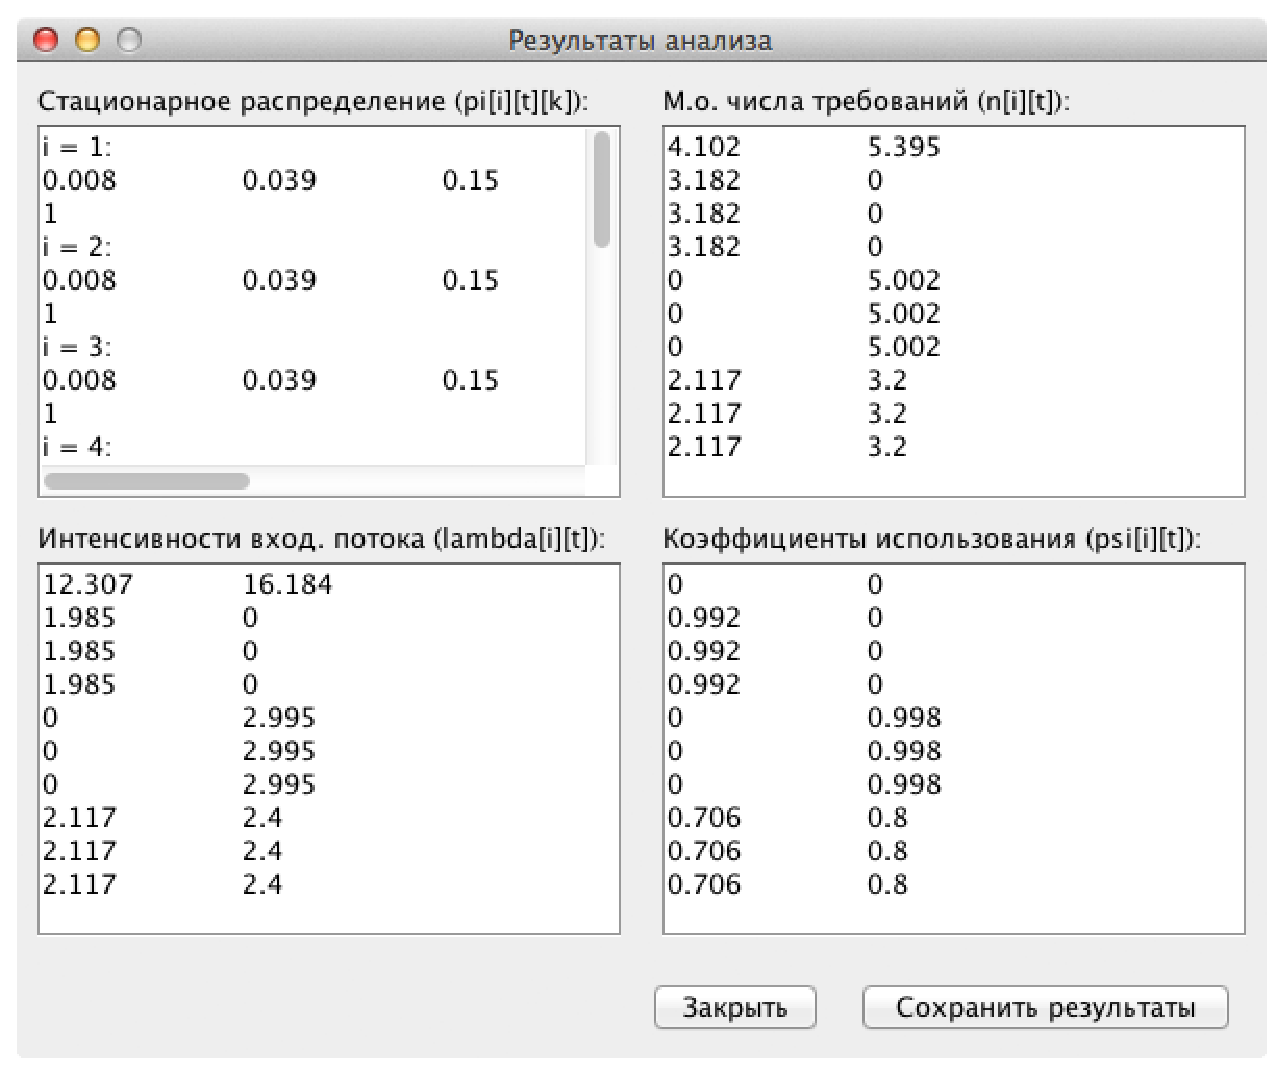
\includegraphics[width=0.8\textwidth]{results}
  \label{fig:main}
\end{figure}
\end{frame}

% ------------------------------------------------------------------- %

\begin{frame} \frametitle{Зависимость стационарных характеристик ГПС от числа приборов}
\begin{figure}[H]
  \centering
  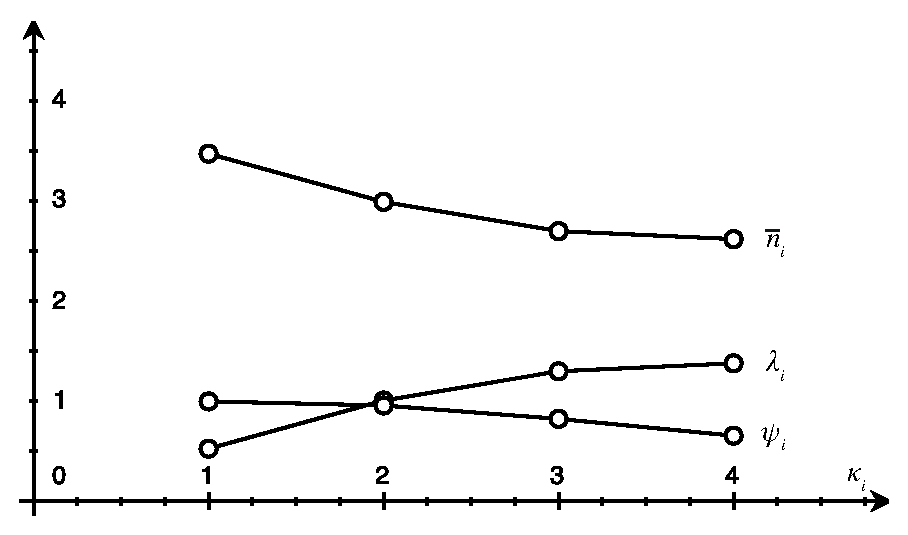
\includegraphics[width=0.9\textwidth]{graph1}
  \label{fig:main}
\end{figure}
\end{frame}

% ------------------------------------------------------------------- %

\begin{frame} \frametitle{Зависимость стационарных характеристик ГПС от емкостей рабочих станций}
\begin{figure}[H]
  \centering
  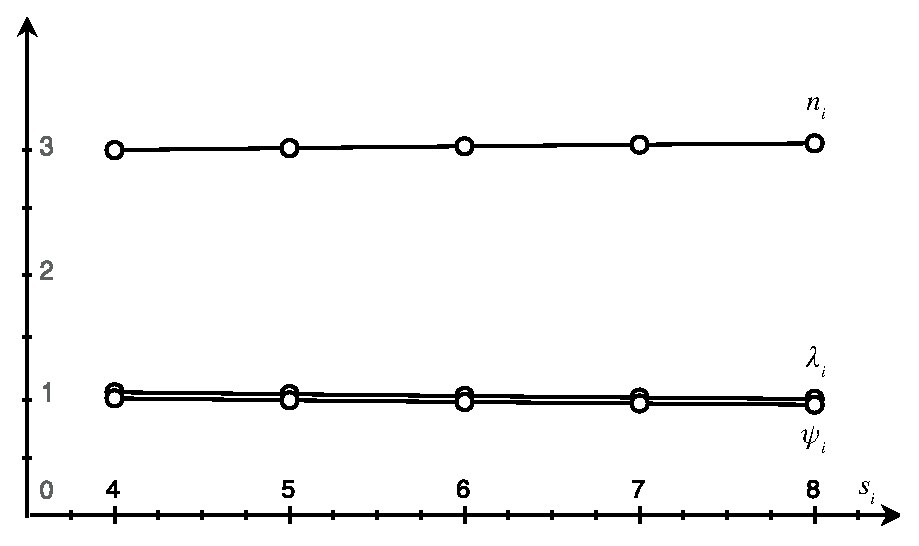
\includegraphics[width=0.9\textwidth]{graph2}
  \label{fig:main}
\end{figure}
\end{frame}

% ------------------------------------------------------------------- %

\begin{frame} \frametitle{Зависимость стационарных характеристик ГПС от интенсивностей обработки деталей}
\begin{figure}[H]
  \centering
  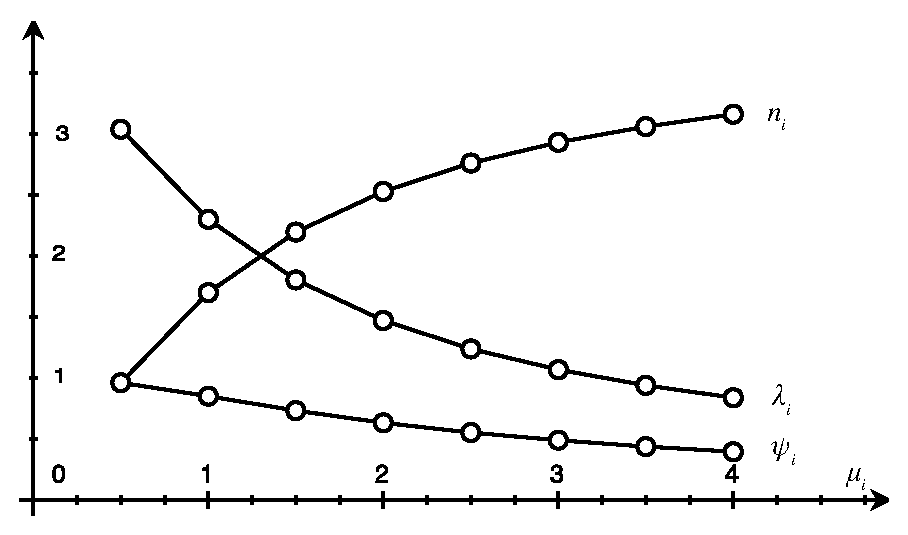
\includegraphics[width=0.9\textwidth]{graph3}
  \label{fig:main}
\end{figure}
\end{frame}
